\section{Problem no.3}
In this last part the aim is to verify the radiating element behavior, starting from the single patch and arriving to the complete array. For the patch antenna we use the one we designed for the second laboratory, that are described in the following image (Figure \ref{patch} shows the patch with the values after the first optimization and figure \ref{patch_mesh} the mesh with the particular of the feeding line).
\begin{figure}[H]
	\centering
	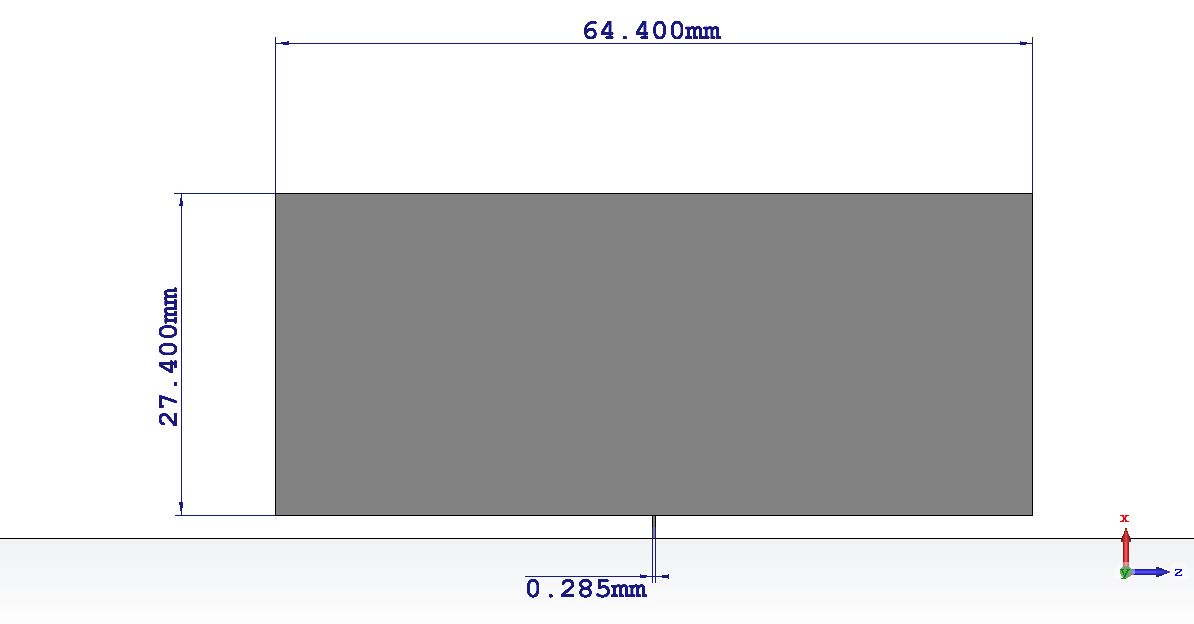
\includegraphics[width=0.9\linewidth]{patch.png}
	\caption{patch resonant at $2.45GHz$}
	\label{patch}
\end{figure}
\begin{figure}[H]
	\centering
	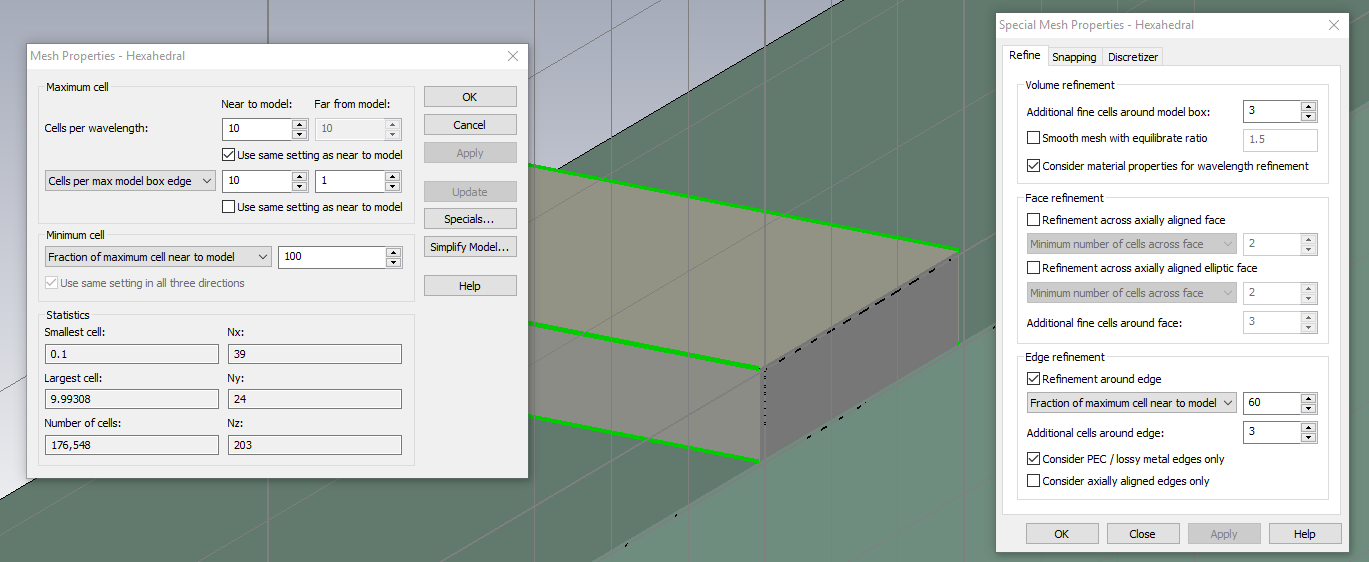
\includegraphics[width=0.9\linewidth]{patch_mesh.png}
	\caption{mesh used for the patch}
	\label{patch_mesh}
\end{figure}

\paragraph{single antenna} First of all we analyze the single antenna itself, so that we control it resonates at the correct frequency with our feeding. We use a very short line with characteristic impedance close to the patch output one, in order to simulate the effective feeding that will be implemented with the beam forming network. This choice is made also to minimize the contribution due to the mismatching of the load the line, and in fact the length of the microstrip feeding is much less than $\lambda$.
\begin{figure}[H]
	\centering
	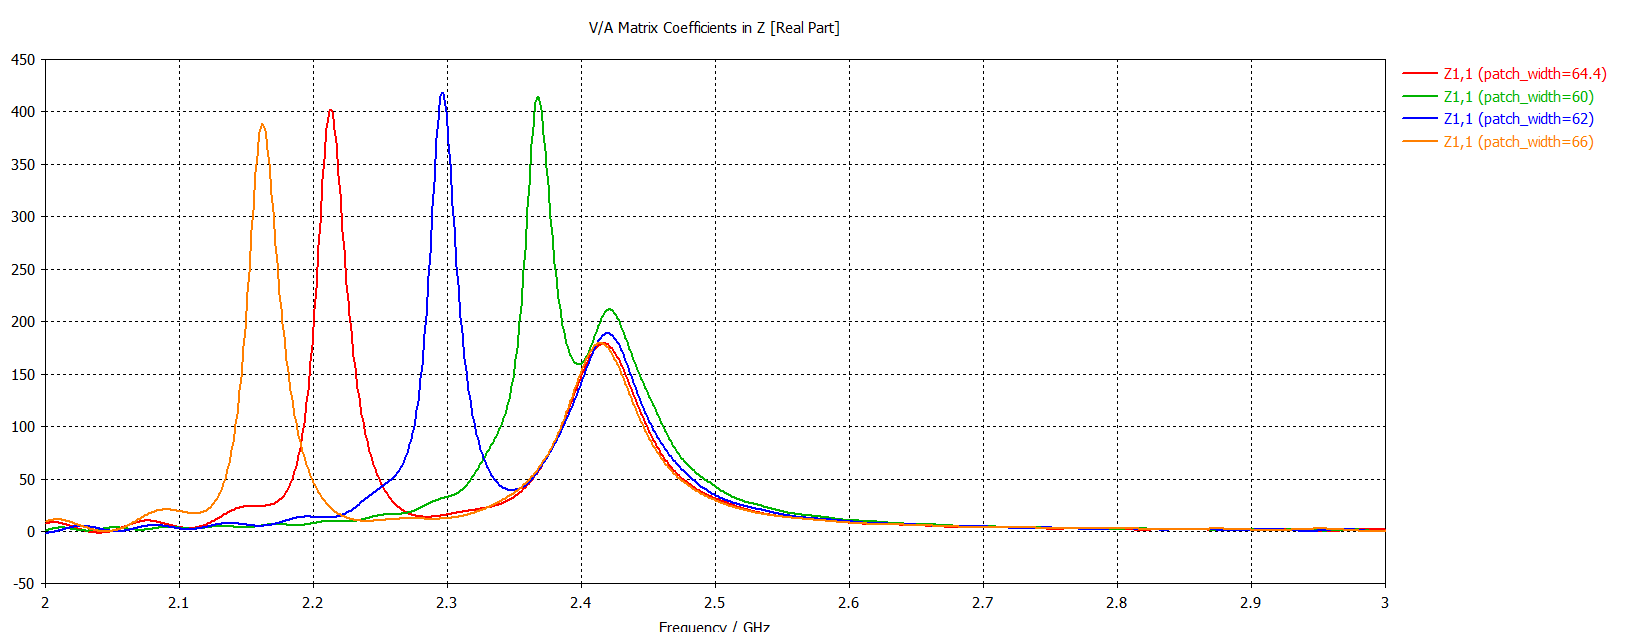
\includegraphics[width=0.9\linewidth]{length_tuning.png}
	\caption{real part of Z11 of the single patch. the parameter that is switching is the width of the antenna}
	\label{length_tuning}
\end{figure}
\begin{figure}[H]
	\centering
	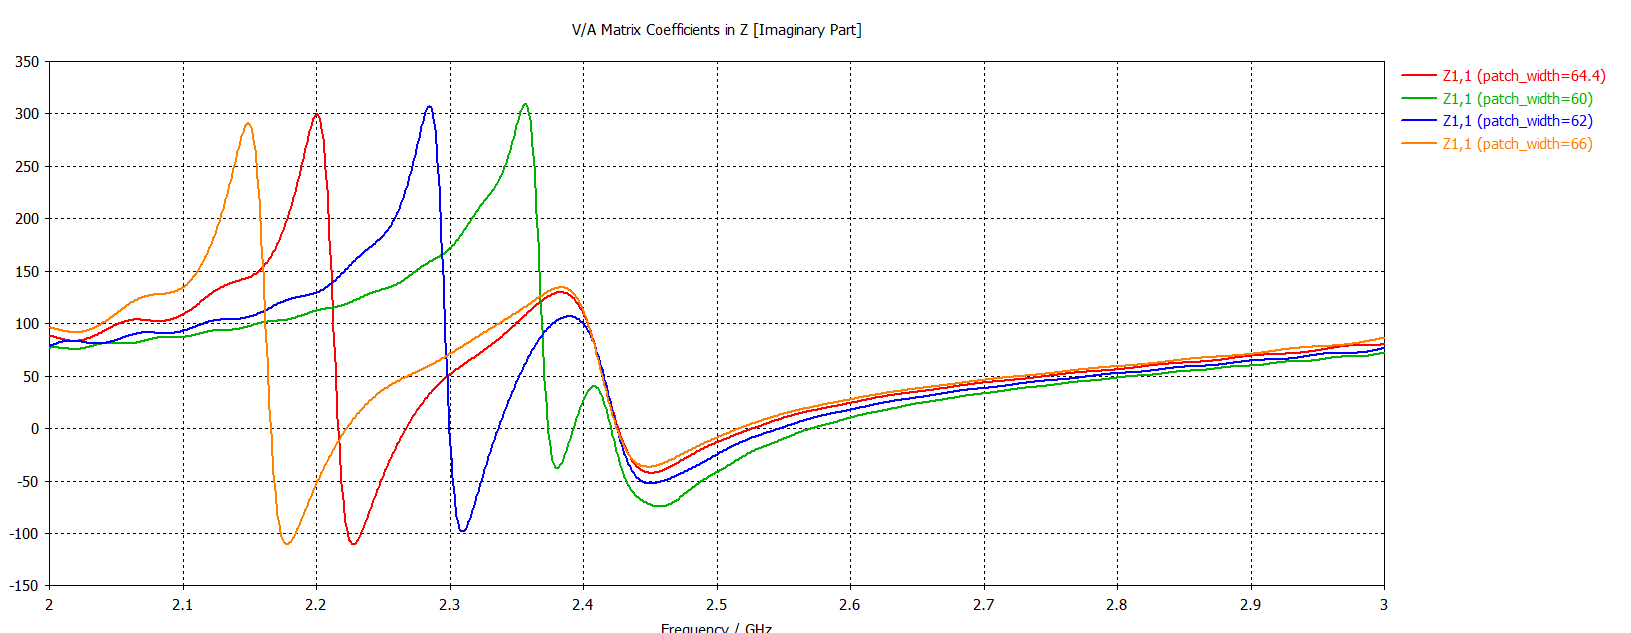
\includegraphics[width=0.9\linewidth]{length_tuning2.png}
	\caption{imaginary part of Z11 of the single patch. the parameter that is switching is the width of the antenna}
	\label{length_tuning2}
\end{figure}
We simulate the antenna scattering parameter, and with this simulation we verify the correct resonance at $2.45GHz$ with an input impedance close to $120\Omega$. On the figure \ref{length_tuning} is possible to see some value of this first simulation. Important to notice that  the impedance is not exactly $120\Omega$. This value is hard to reach and tends to block at almost $160\Omega$ when the width is near to $64.4mm$. On the other side as we can see on figure \ref{length_tuning2} the resonance is a bit before the wanted frequency, but in this case we don't want to optimize the length before simulating the inter elements effects (those contribution could increase the resonance frequency).

\begin{figure}[H]
	\centering
	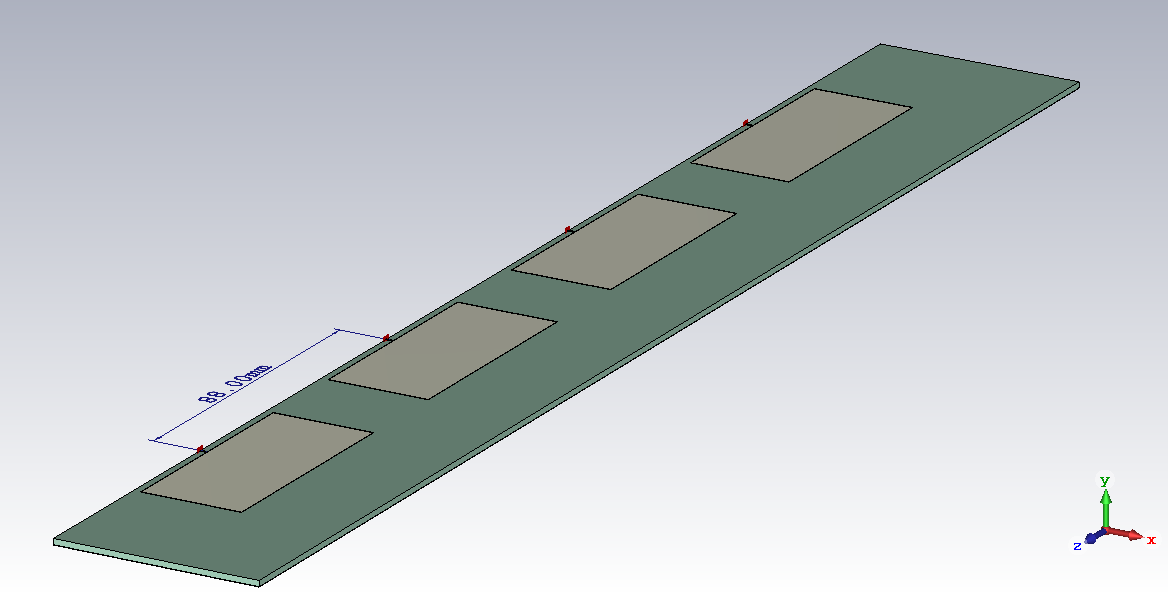
\includegraphics[width=0.9\linewidth]{array.png}
	\caption{patch resonant at $2.45GHz$}
	\label{array}
\end{figure}

\paragraph{multiple antennas} Composing the array with those antennas we can have a first simulation of the complete radiating element, and so we can make some considerations. The bigger issue in particular are the resonance frequency, which due to the inter elements coupling (as expected) are deviated from the single antenna case. In particular the resonance frequency results shifted of few hundreds of megahertz upward, movement that we have to take in mind in case we want to re-design a similar patch antenna complying better with the specifications.
\begin{figure}[H]
	\centering
	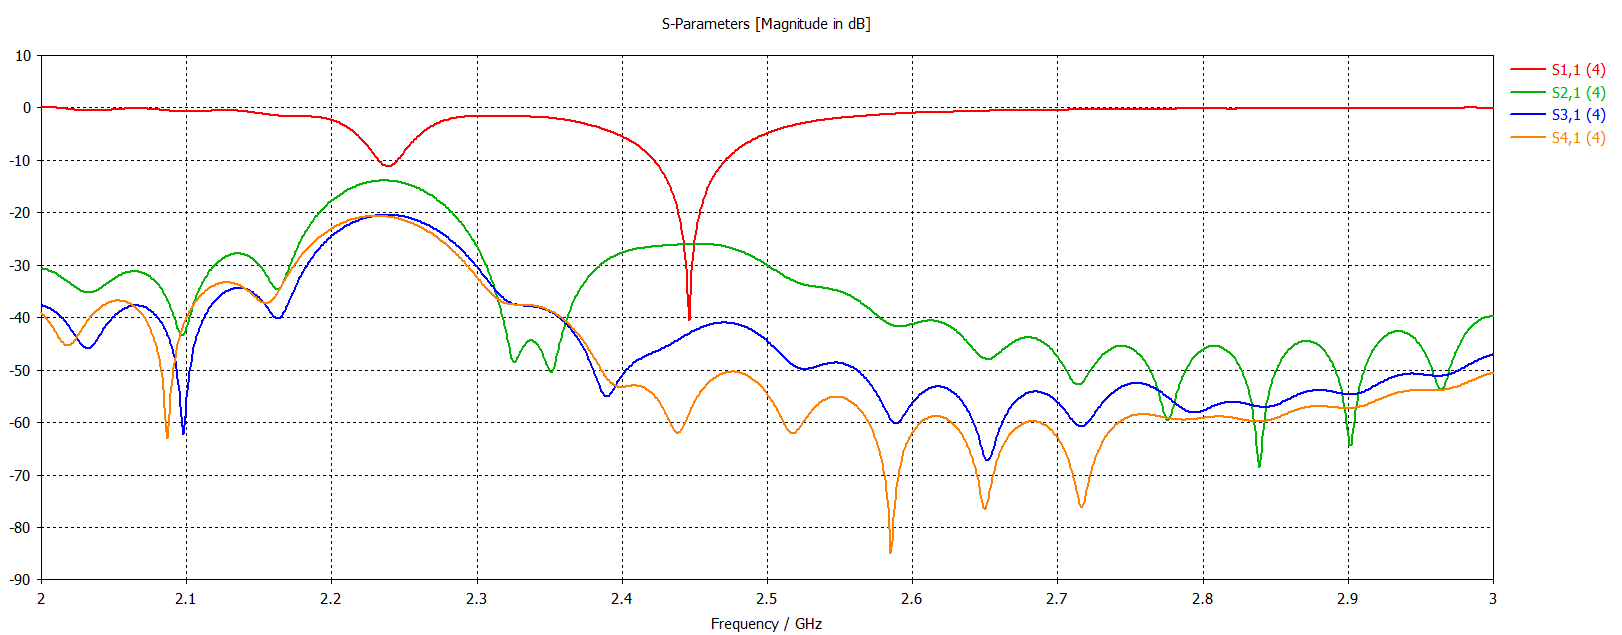
\includegraphics[width=0.9\linewidth]{scattering_array.png}
	\caption{all the scattering parameters with feeding on port 1}
	\label{scattering_array}
\end{figure}
Simulating the four antennas with their entering ports we have a total number of 16 scattering parameters, which are not so easy to handle in order to find the load seen from the beam forming network point of view and optimize it. Because we use a constant tapering for the antennas feeding we can combine the results of this simulation and find only four scattering parameters describing the reflection coefficient of each port. This way we can also find the correlated impedance, so that in our particular case of feeding we can evaluate precisely the active impedance of the antennas. The value founded using the tapering evaluated in the previous parts of the design are showed in the figures \ref{array_real} and \ref{array_imm}
\begin{figure}[H]
	\centering
	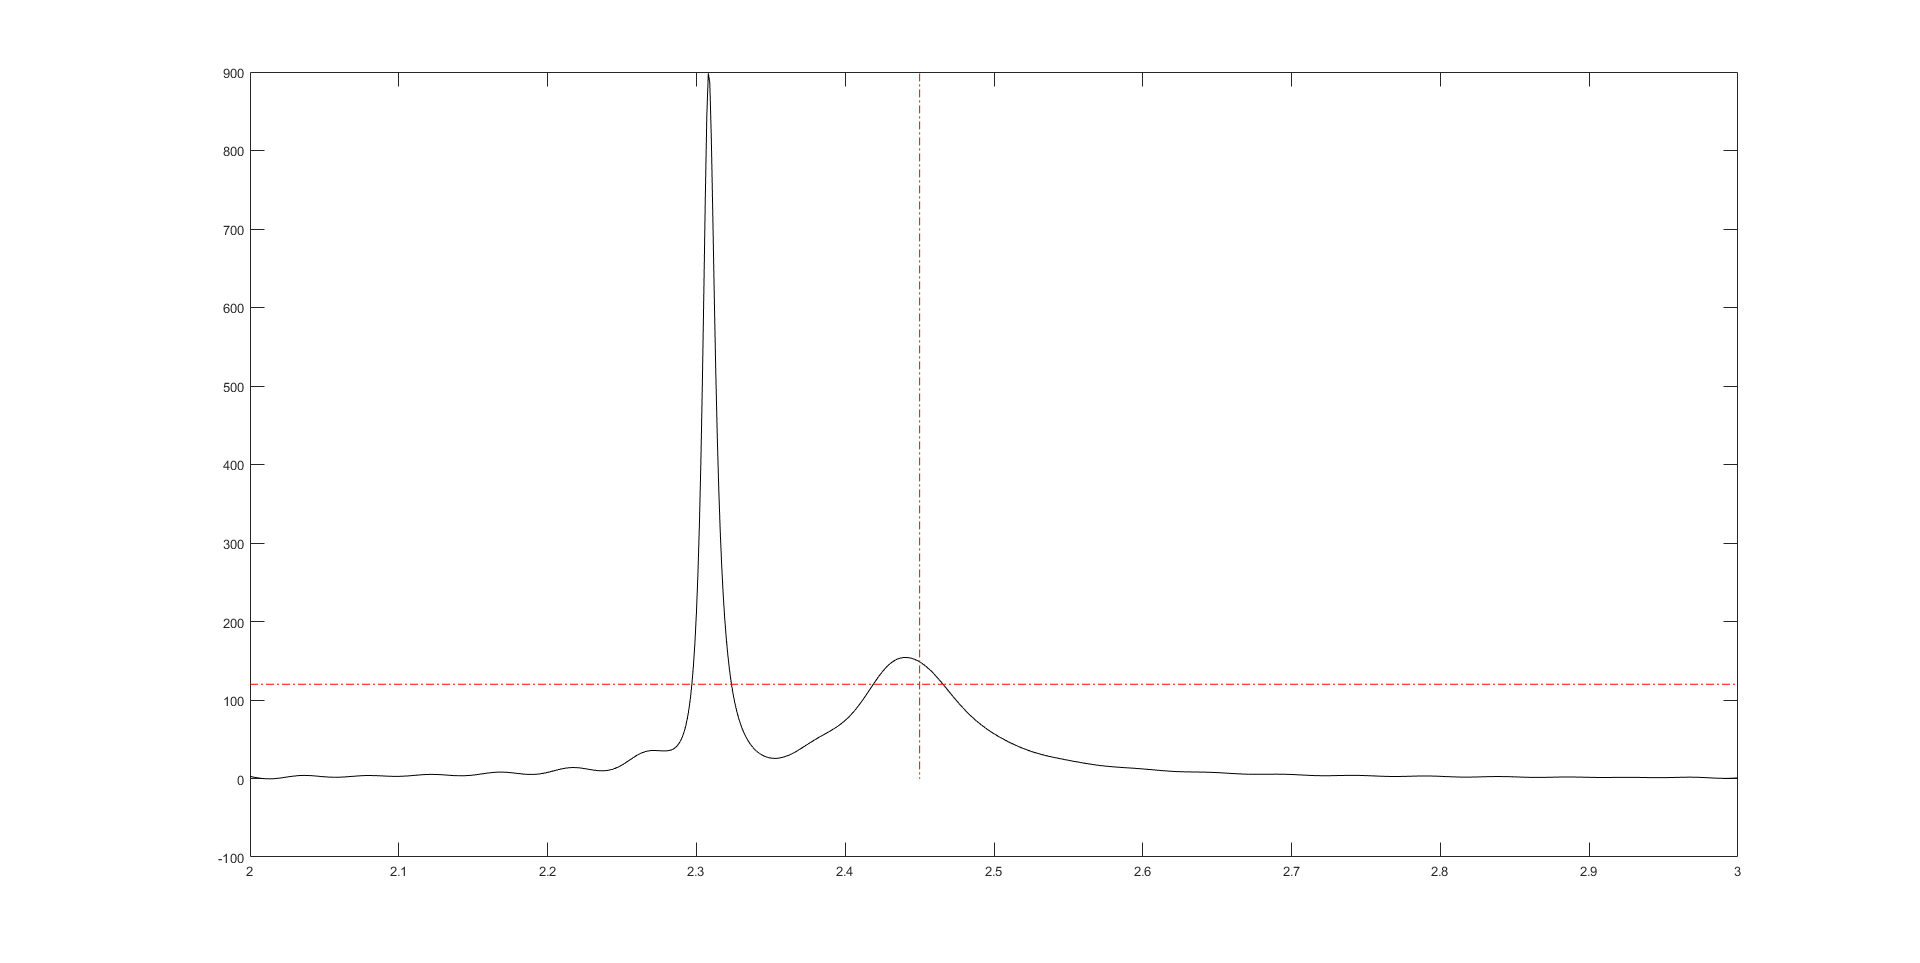
\includegraphics[width=0.9\linewidth]{array_real.png}
	\caption{real part of Z11 of the array}
	\label{array_imm}
\end{figure}
\begin{figure}[H]
	\centering
	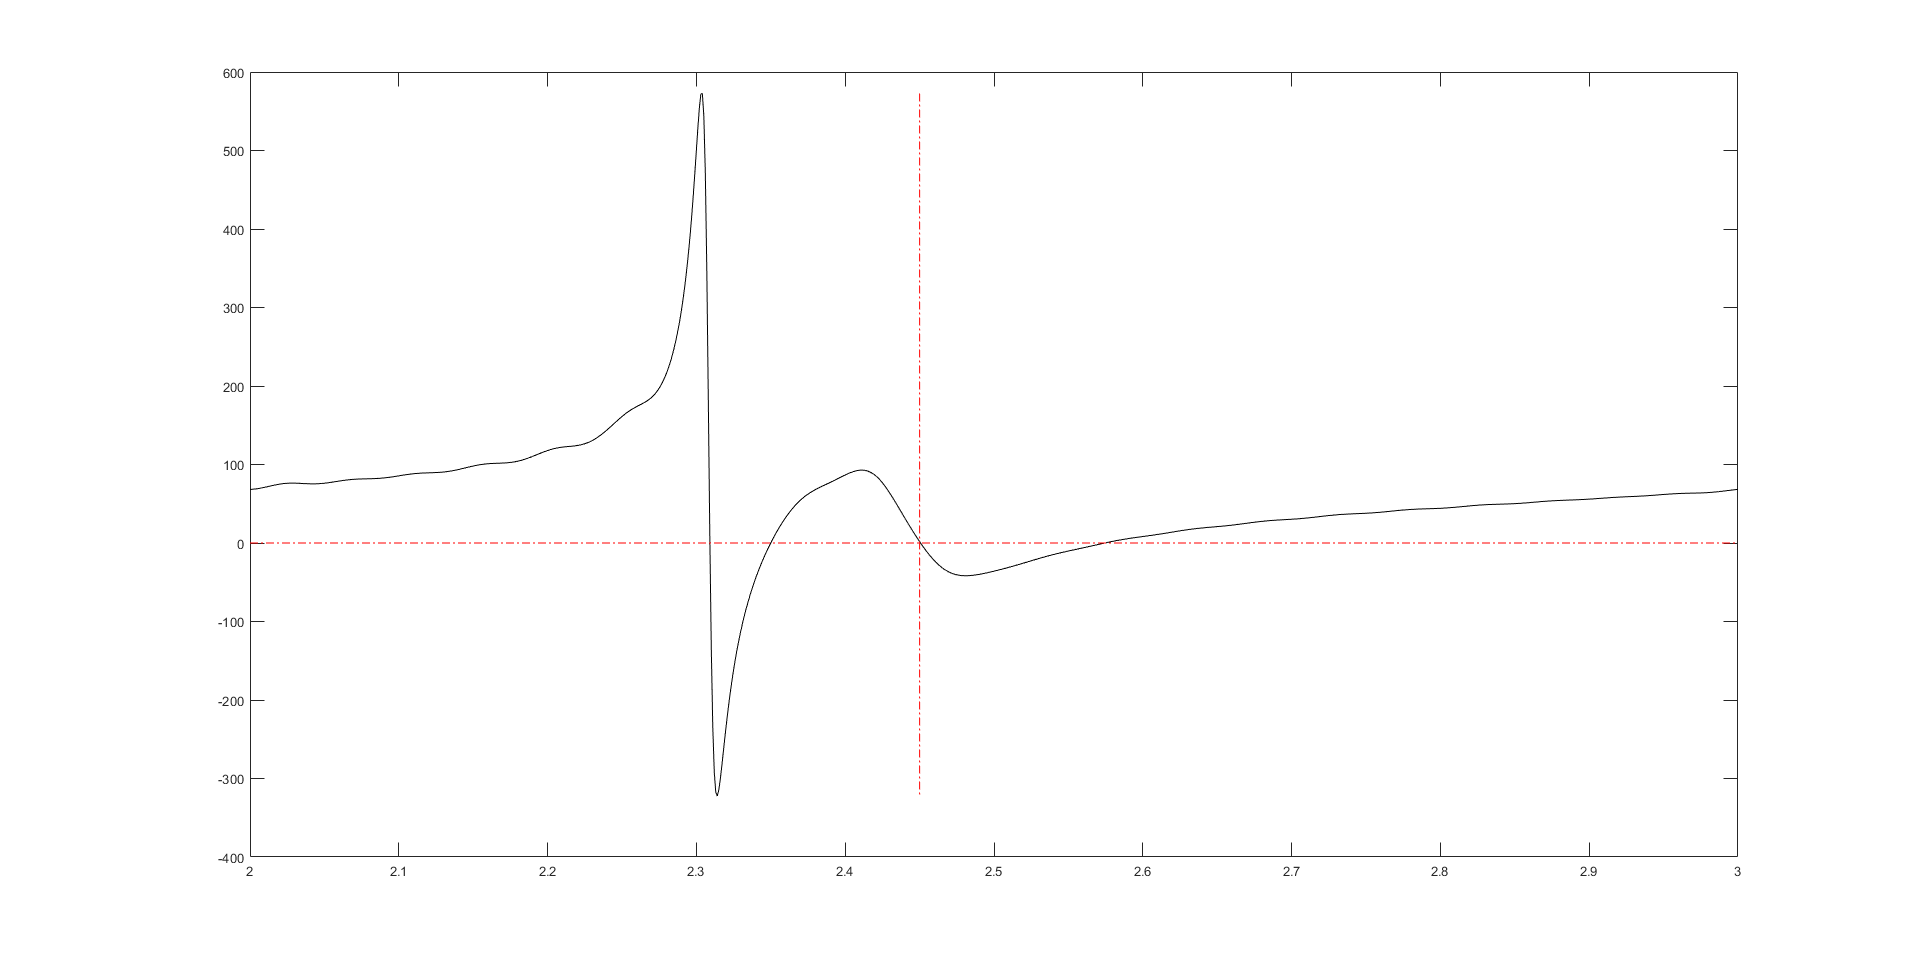
\includegraphics[width=0.9\linewidth]{array_imm.png}
	\caption{imaginary part of Z11 of the array}
	\label{array_real}
\end{figure}
Cause of the symmetry of the structure we have that the impedance of the external elements should slightly differs from the internal one, but as we can see on the scattering parameters on the figure \ref{array_scat} the differences are negligible. On top of that we can finally observe, concerning the scattering parameters, that at the wanted frequency we have less than -20dB matching.
\begin{figure}[H]
	\centering
	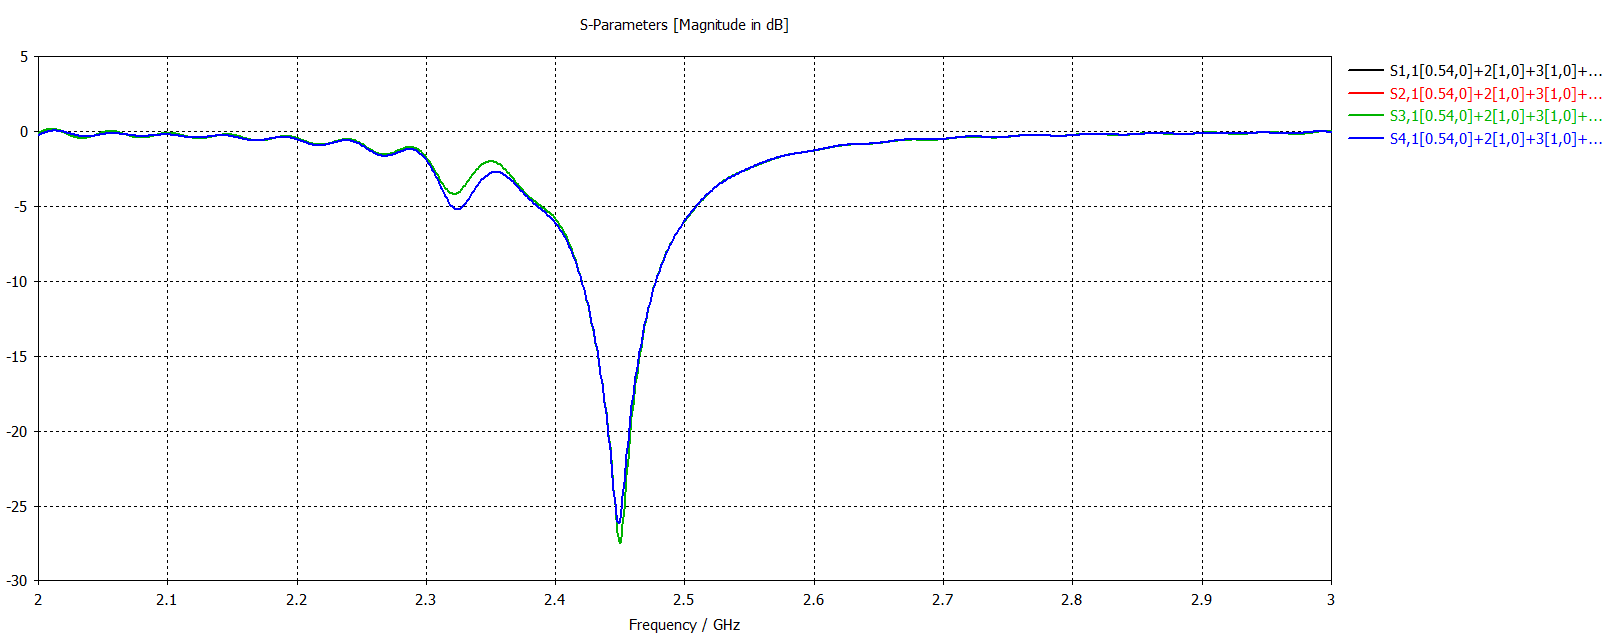
\includegraphics[width=0.9\linewidth]{array_scat.png}
	\caption{scattering parameters of the array}
	\label{array_scat}
\end{figure}

\paragraph{array factor} The last pass is to consider the radiation pattern, which is first of all evaluated with a far field monitor, and after that is exported and elaborated in Matlab in order to verify the correct behavior of the array factor. For this calculation we need also the far field radiation of the single patch antenna, which must be used as a punctual divider for the array far field.
\begin{lstlisting}
% import of the data from file exported in ASCII from CST
data_file='data.txt';
data=fopen(data_file,'r');
fgets(data);
fgets(data);
data_val=fscanf(data,'%f %f %f %f %f %f %f %f',[8 Inf]);
[~,len]=size(data_val);
fclose(data);
% prev_val is the set of value taken at the first read, which in our case
% is the radiation pattern of the array
figure(1) % rad array
plot(prev_val(1,:),prev_val(3,:),'k',[prev_val(1,1) prev_val(1,len)],[0 0],'-.r',[2.45 2.45],[min(prev_val(3,:)) max(prev_val(3,:))],'-.r')
figure(2) % rad patch
plot(data_val(1,:),data_val(3,:),'k',[data_val(1,1) data_val(1,len)],[0 0],'-.r',[2.45 2.45],[min(data_val(3,:)) max(data_val(3,:))],'-.r')
figure(3) %AF
plot(data_val(1,:),prev_val(3,:)-data_val(3,:),'k',[data_val(1,1) data_val(1,len)],[-20 -20],'-.r',[90 90],[-40 max(data_val(3,:))],'-.r')
\end{lstlisting}
The result of this calculation is the array factor printed in figure \ref{rad_pattern_AF}, which does not respect the initial requirements for the side lobes (only less than -$15dB$) and the grating lobes (which are evident and arrives at $-5dB$). This optimization, as the one in the previous point, is very long and requires a lot of calculation, so we have to accept this as the best result. Regarding all the other characteristic, the array is verified to work in broadband, and the bandwidth at $-3dB$ is $16^{\circ}$.
\begin{figure}[H]
	\centering
	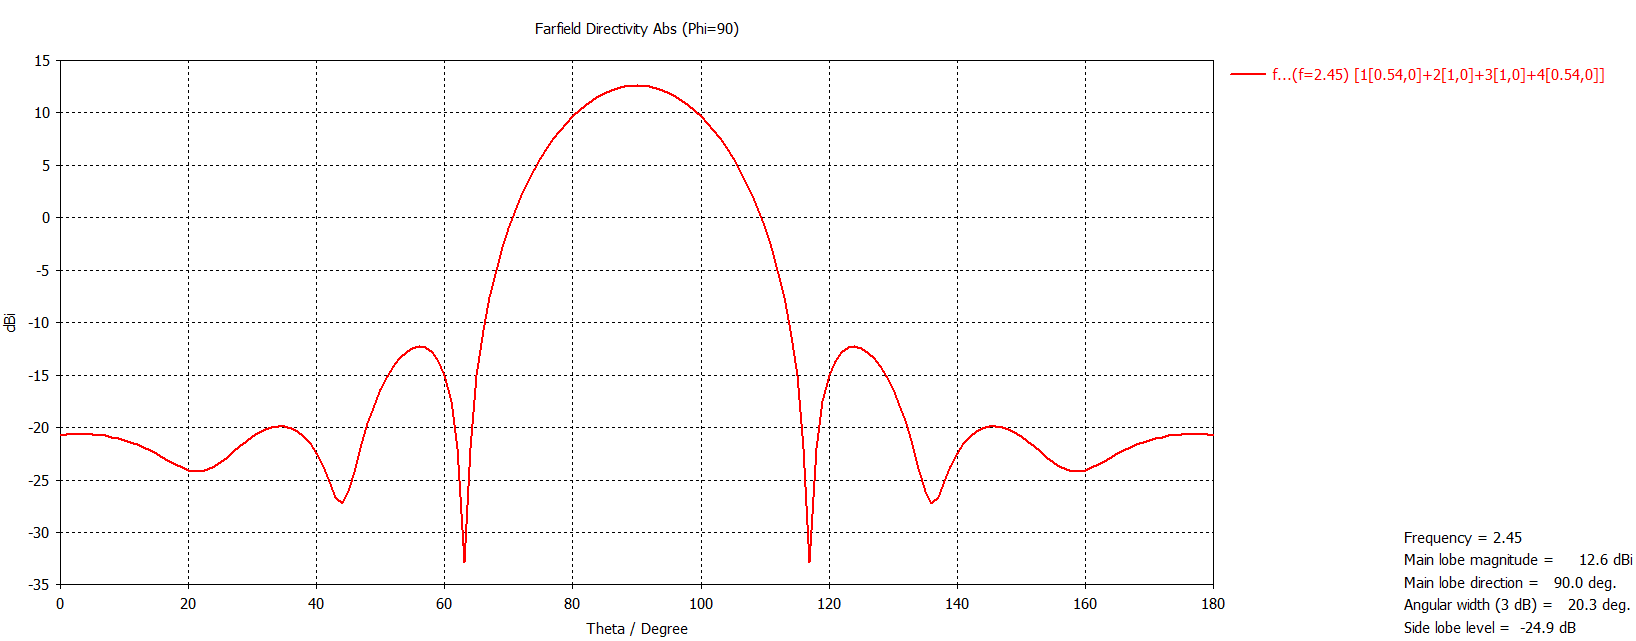
\includegraphics[width=0.9\linewidth]{rad_pattern_array.png}
	\caption{radiation of the array}
\end{figure}
\begin{figure}[H]
	\centering
	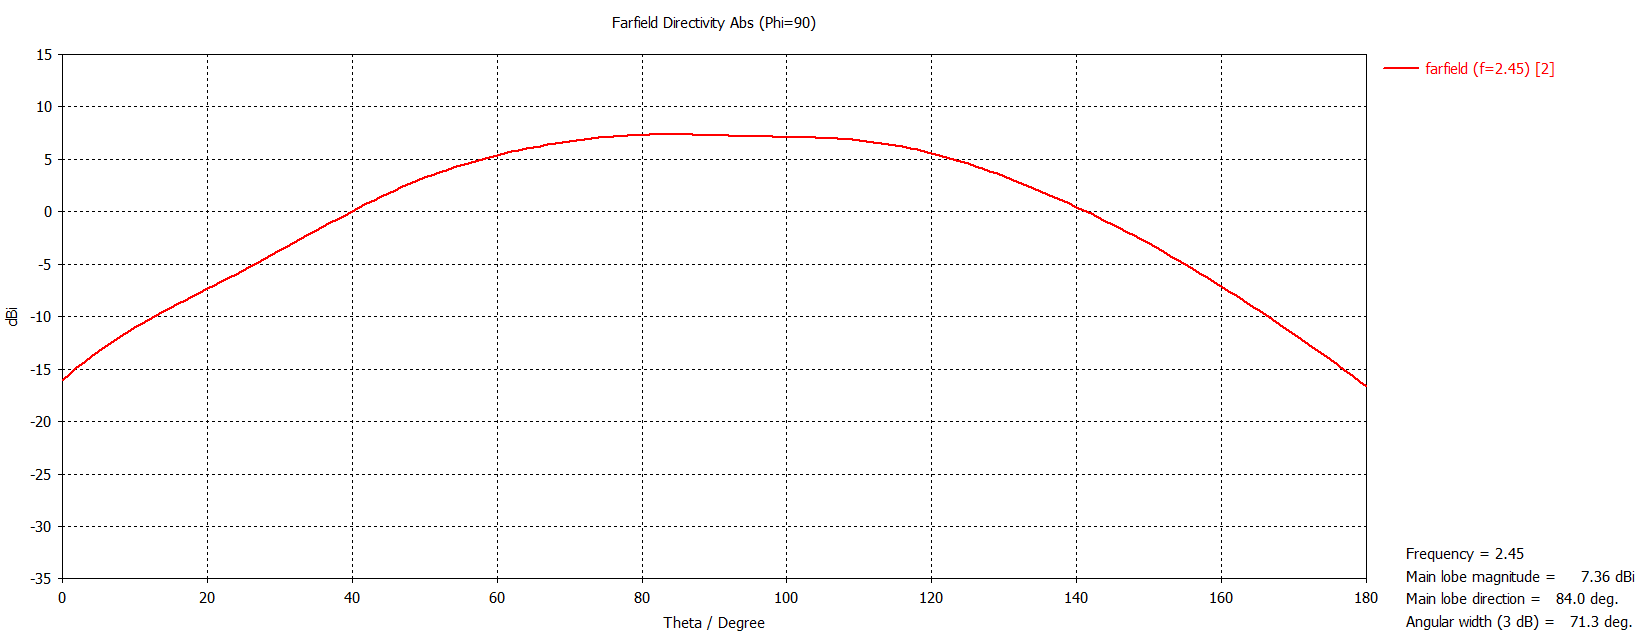
\includegraphics[width=0.9\linewidth]{rad_pattern_patch.png}
	\caption{radiation of the single patch}
\end{figure}
\begin{figure}[H]
	\centering
	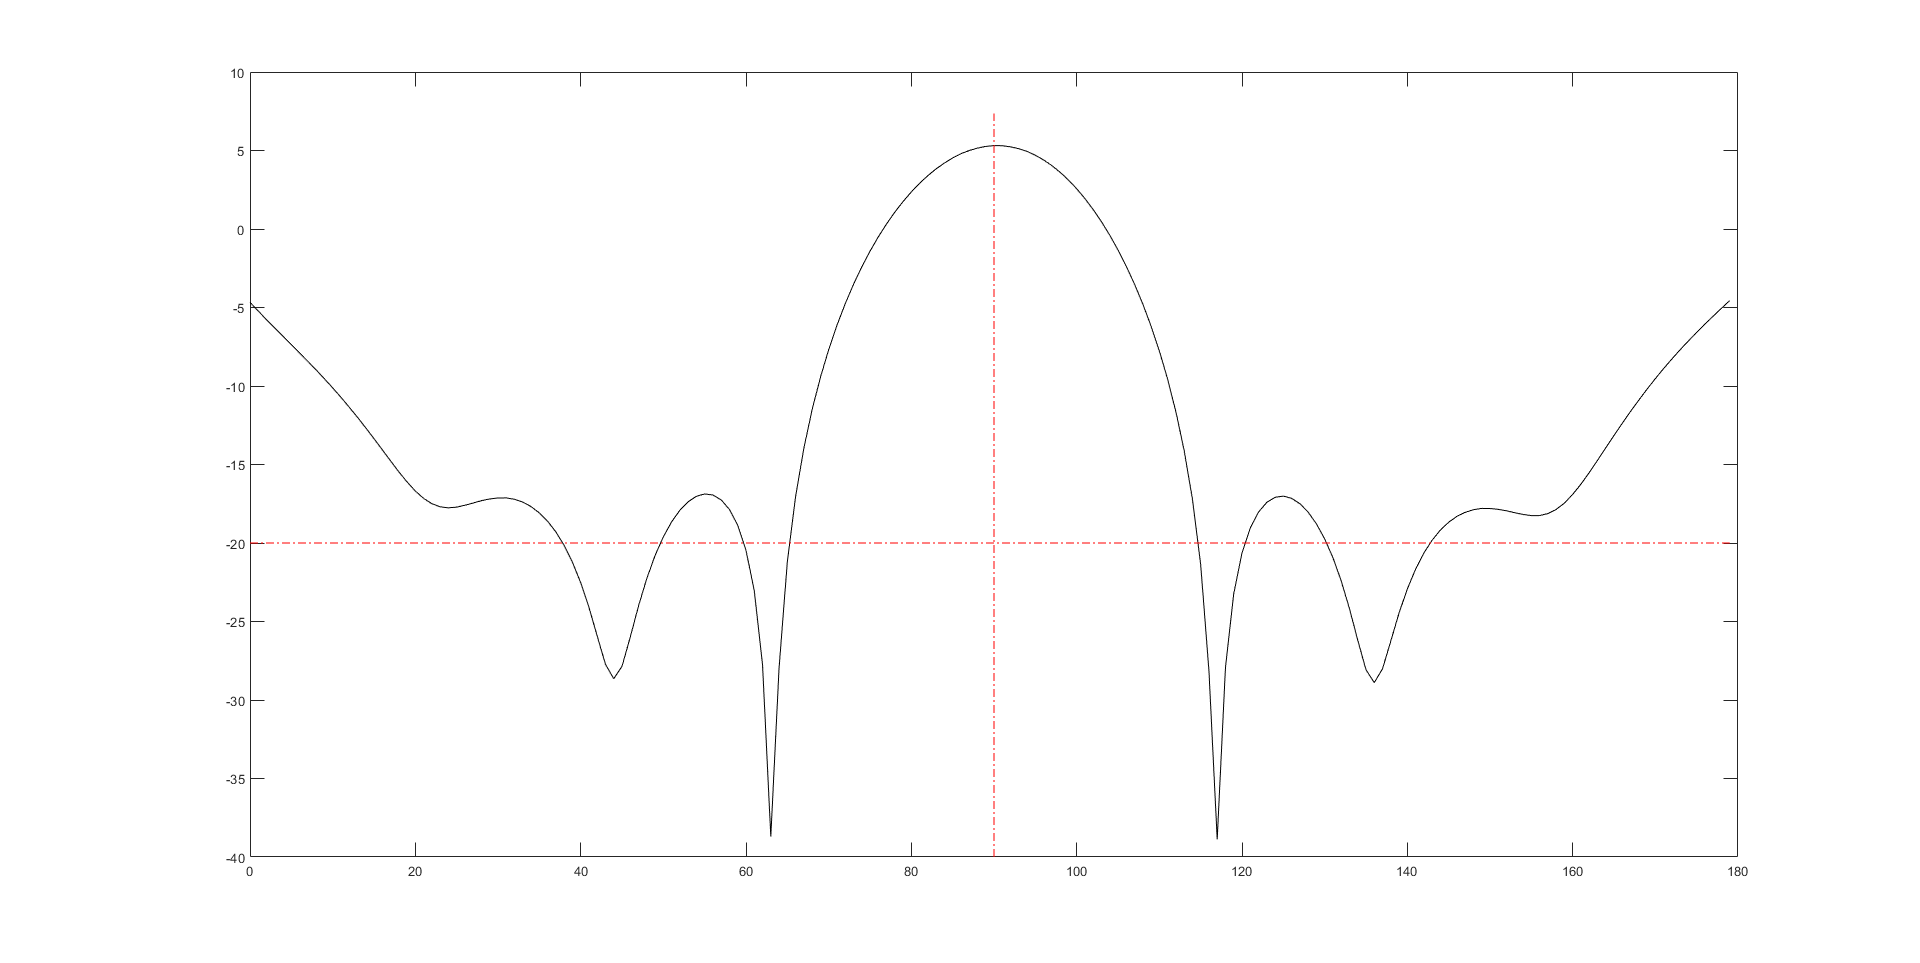
\includegraphics[width=0.9\linewidth]{rad_pattern_AF.png}
	\caption{antenna factor of the array}
	\label{rad_pattern_AF}
\end{figure}